\chapter{Campi elettrici}
\section {L'aspetto fisico}
La forza elettrostatica tra 2 cariche sembra una ``azione a distanza''
\begin{itemize}
\item Spiegazione alternativa:\\
  \textit{La carica 1 crea un campo elettrico nello spazio circostante}\\
  \textit{La carica 2 sente l'effetto del campo 1}\\
\item vice versa:\\
  \textit{La carica 2 crea un campo elettrico nello spazio circostante}\\
  \textit{La carica 1 sente l'effetti del campo 2}
\end{itemize}
\section {Il campo elettrico}
\begin{tasks}{2}
\task campo scalare: temperatura, pressione, densità
\task campo vetoriale: velocità, accelerazione, forza
\end{tasks}
La forza $\vec{F}$ su un \textbf{carica esplorativa} $q_0$ determina il campo elettrico $\vec{E}$:
\begin{equation}
  \vec{E}=\frac{\vec{F}}{q_0}
\end{equation}
$\vec{E}$ è un campo vettoriale. Nel SI ``Sistema Internazione'', si esprime in N/C (o V/m)
\section{Linee di campo elettrico}
Per visualizzare $\vec{E}$, disegnamo delle linee:
\begin{itemize}
	\item Il vettore $\vec{E}$ è \textbf{tangente} alla linea 
	\item La \textbf{densità} delle linee rappresenta $\abs{\vec{E}}$
        \item Le linee \textbf{escono} dalle cariche positive
        \item Le linee \textbf{entrano} nelle cariche negative
\end {itemize}
\section {Altro esempio delle linee di campo}
\begin{figure}[!h]
 	\centering
	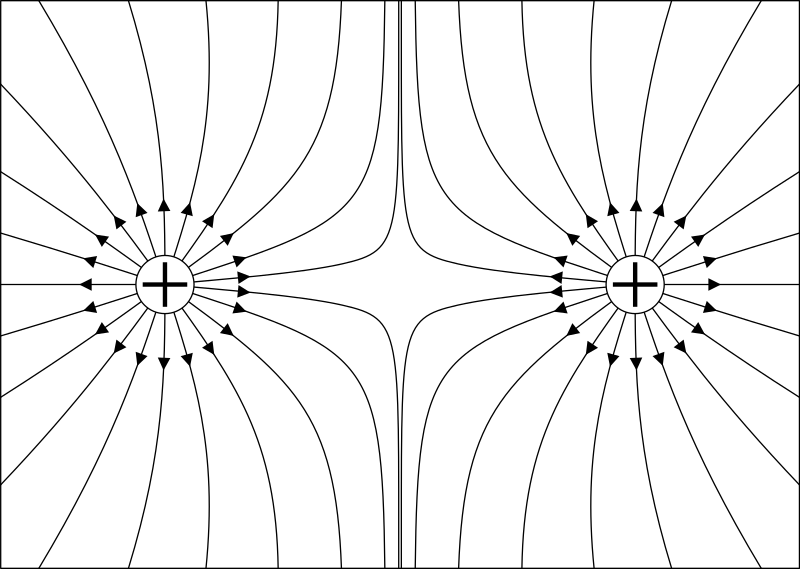
\includegraphics[height=4cm]{img/linee elettriche repulsione.png}
\end{figure}
Due cariche positive identifiche\\
Sempre:
\begin{itemize}
\item Il vettore $\vec{E}$ è tangente alla linea
\item La densità delle linee rappresenta $\abs {\vec{E}}$
\item Le linee escono dalla cariche positive
\item Le linee entrano nelle cariche negative
\end{itemize}
Il disegno stesso suggersce l'idea di una repulsione
\section{Campo $\vec{E}$ di una carica puntiforme}
Una carica esploratrice positiva $q_0$ attorno ad una \textit{carica puntiforme} $q$ sente una forza $\vec{F}=\frac{qq_0}{4\pi \xi_0r^2}\hat{r}$. \\
Per il campo $\vec{E}$ troviamo:
\begin{equation}
	\vec{E}=\frac{\vec{F}}{q_0}=\frac{q}{4\pi \xi_0r^2}\hat{r}
\end{equation}
La direzione di $\vec{E}$ è \textbf{radiale}
\begin{enumerate}
\item Per $q>0$, il verso di $\vec{E}$ è uscente
\item Per $q<0$, il verso di $\vec{E}$ è entrante
\end{enumerate}
Per il \textbf{modulo:} $E=\abs{\vec{E}}=\frac{\abs q}{4\pi \xi_0r^2}$  
\section{Il principio di sovrapposizione}
In presenza di \textbf{più cariche}, le forze obbediscono al principio di sovrapposizione:
\begin{equation}
  \vec{F}_0=\vec{F}_{01}+\vec{F}_{02}+\dots+\vec{F}_{0n}
\end{equation}
Il principio di sovrapposizione vale anche per $\vec{E}$:
\begin{equation}
  \vec{E}=\frac{\vec{F}_0}{q_0}+\frac{\vec{F}_{01}}{q_0}+\frac{\vec{F}_{02}}{q_0}+\dots+\frac{\vec{F}_{0n}}{q_0}=\vec{E}_1+\vec{E}_2+\dots+\vec{E}_n
\end{equation}
Il campo $\vec{E}$ di più particelle cariche è la somma vettoriale dei singoli contributi
\section{Verifica}
\begin{center}
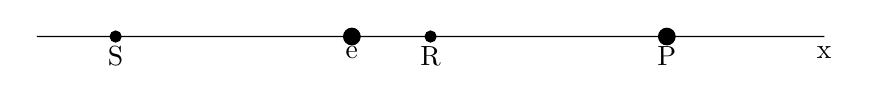
\begin{tikzpicture} 
 \filldraw 
(0,0) circle (0pt) node[align=left,   below] {}      --
(1,0) circle (2pt) node[align=center, below] {S}     -- 
(4,0) circle (3pt) node[align=right, below] {e}     -- 
(5,0) circle (2pt) node[align=right,  below] {R}     --
(8,0) circle (3pt) node[align=right, below] {P}     --
(10,0) circle (0pt) node[align=left, below] {x};
\end{tikzpicture}
\end{center}
Il disegno mostra un elettrone ($e$) e un protone ($p$) sull'asse $x$
\begin{itemize}
	\item Indicare la direzione di \textit{E} dovuta all’elettrone nel
           punto \textit{S} e nel punto \textit{R}
        \item Indicare la direzione di \textit{E} dovuta al protone nel
punto \textit{S} e nel punto \textit{R}
\end{itemize}
\subsection {Soluzione}
\begin{equation}
  \begin{matrix}
    q_1=+2e\\
    q_2=-2e\\
    q_3=-4e
  \end{matrix}
\end{equation}
Ovviamente il primo passo da fare è quello di ricavare $\vec{E}$ nel origine
\begin{equation}
  E_1=E_2=\frac{2e}{4\pi\xi_0d^2}
\end{equation}
\begin{equation}
	E_3=\frac{4e}{4\pi\xi_0d^2}
\end{equation}
Ora ricaviamo $E_x$ tramite una somma tra $E_{1x}$, $E_{2x}$ e $E_{3x}$.
\begin{equation}
	E_x=E_{1x}+E_{2x}+E_{3x}=\frac{2e}{4\pi\xi_0d^2}\cos{30^o}+\frac{2e}{4\pi\xi_0d^2}\cos{30^o}+\frac{4e}{4\pi\xi_0d^2}\cos{30^o}=\frac{8e}{4\pi\xi_0d^2}\cos{30^o}
\end{equation}
\begin{equation}
	E_x=E_{1y}+E_{2y}+E_{3y}=\frac{-2e}{4\pi\xi_0d^2}\cos{30^o}+\frac{-2e}{4\pi\xi_0d^2}\cos{30^o}+\frac{4e}{4\pi\xi_0d^2}\cos{30^o}=0
\end{equation}
\section{Campo $\vec{E}$ di un dipolo elettrico}
Due particelle cariche, $-q$ e $+q$ separate da distanza $d$ e sull'asse dipolare $z$. Il prodotto $qd$ viene chiamato \textbf{momento di dipolo elettrico}: $p=qd$ e $\vec{p}$ vettoriale.
\begin{itemize}
\item direzione: l'asse dipolare
\item verso: da $-q$ a $+q$
\end{itemize}
Il campo $\vec{E}$ sull'asse dipolare distante $z$ dal centro del dipolo:
\begin{equation}
  \begin{matrix}
    E=E_+-E_-=\frac{q}{4\pi \xi\left(z-\frac{d}{2}\right)^2}-\frac{q}{4\pi \xi\left(z-\frac{d}{2}\right)^2}
    =\frac{q}{4\pi\xi_0}\frac{\left(z-\frac{d}{2}\right)^2-\left(z-\frac{d}{2}\right)^2}{\left(z-\frac{d}{2}\right)^2\left(z-\frac{d}{2}\right)^2}
    =\frac{q}{4\pi\xi_0}\frac{2zd}{\left(\left(z-\frac{d}{2}\right)^2\right)^{2}}\\
    =\frac{qd}{2\pi\xi_0z^3}\left(1-\left(\frac{d}{2z}\right)^2\right)^{-2}
    \end{matrix}
\end{equation}
Per $z>>d$ troviamo $E(z)=\frac{p}{2\pi\xi_0z^3}$, anche fuori dell'asse $z$, $E\propto r^{-3}$ per $r>>d$\\
Materiale isolandte (\textbf{e. g. plastica}). Raggio \textit{R}, carica \textbf{superficiale} $\sigma$ - Punto \textit{P} sull'asse centrale, direzione \textit{z}. Ogni anello ha carica $dq=\sigma 2\pi rdr$ e contribuisce a $dE=\frac{zdq}{4\pi\xi_0\left(4r^2+z^2\right)^{\frac{3}{2}}}$
\begin{equation}
  E=\inf dE=\int^R_0\frac{z\sigma2\pi rdr}{4\pi\xi_0\left(4r^2+z^2\right)^{\frac{3}{2}}}=\frac{z\sigma}{4\xi_0}\left[\frac{\left(4r^2+z^2\right)^{-\frac{1}{2}}}{-\frac{1}{2}}\right]^R_0
\end{equation}
Il risultato è $E=\frac{\sigma}{2\xi_0}\left(1-\frac{z}{\sqrt{R^2+z^2}}\right)$. Per $z<<R$ troviamo $E=\frac{\sigma}{2\xi_0}$.\\
Su una carica $q$ in un campo elettrico esterno $\vec{E}$ agisce un forza elettrostatica $\vec{F}=q\vec{E}$
\begin{itemize}
  \item per $q>0$, $\vec F$ ha lo stesso orientamento di $\vec E$
  \item per $q<0$, $\vec F$ ha l'orientamento opposto di $\vec E$
\end{itemize}
NB: Una carica non sente il proprio campo elettrico esterno!
\section{Misura della carica elementare}
\subsection{Millikan 1910}
\fbox{
 	\addtolength{\linewidth}{-2\fboxsep}%
 	\addtolength{\linewidth}{-2\fboxrule}%
	\begin{minipage}{\linewidth}
          L'esperimento di Millikan per antonomasia è l'esperimento della goccia d'olio, il cui obiettivo, cioè
          misurare la carica elettrica dell'elettrone, fu raggiunto nel 1909. Il valore ricavato da Robert
          Millikan fu $4,774(5) x 10^{-10}$ statcoulomb, equivalenti a $1,5924(17)x10^{-19}$ coulomb, minore
          dello 0,6\% circa rispetto a quello oggi comunemente accettato, pari a $1,602176634 x 10^{-19}$ coulomb.
        \end{minipage}
}
\begin{center}
  \href{https://it.wikipedia.org/wiki/Esperimento_di_Millikan}{By Wikipedia}
\end{center}
\subsubsection{Problema svolto}
Una goccia con $m=1,3*10^{-10}$, $Q=-1,5*10^{-13}C$ e $V_x=18m/s$ attraverso una zona di lunghezza $L=1,6cm$ e campo elettrico $E=1,4*10^6N/C$ verso il basso,
Qual'è la deflessione verticale?
\begin{equation}
  y=\frac{1}{2}at^2=\frac{1}{2}\frac{EQ}{m}\left(\frac{L}{vx}\right)^2=6,4*10^{-4}m=0,64mm
\end{equation}
\section{Prodotto scalare}
Esistono due prodotti tra vettori: il \underline{prodotto calare} e il \underline{prodotto vettoriale}.\\
Il prodotto scalare è appunto uno scalare (un \textbf{singolo numero}) funzione di due vettori, indicato con
$s=\vec{A}*\vec{B}$ e perciò anche detto \textbf{dot product}. Operativamente, posto $\abs{A}$ il modulo del vettore $\vec{A}$, $\abs{B}$ il modulo del vettore $\vec{B}$, e $\alpha$ l'\textbf{angolo} compreso tra i due vettori, il prodotto scalare si calcola con
\begin{equation}
	s=\vec{A}*\vec{B}=\abs{\vec{A}}\abs{\vec{B}}\cos \alpha
\end{equation}
Oppure equivalentemente, poste $A_x$ ecc. le componenti dei vettori comme la somma e i prodotti delle componenti
omologhe
\begin{equation}
  \vec{A}*\vec{B}=A_xB_x+A_yB_y+A_zB_z
\end{equation}
L'interpretazione geometrica è che il prodotto scalare è la \textbf{proiezione} di uno dei due vettori
sull'altro.
\section{Prodotto vettoriale}
Il prodotot vettoriale è un vettore funzione di due vettori, è si indica con $\vec{V}=\vec{A}*\vec{B}$ oppove
$\vec{V}=A\textturnv \vec{B}$. È anche detto \textbf{cross product}. Il modulo
$\abs{\vec{V}}=\vec{A}*\vec{B}\sin0$.\\
$\vec{V}$ è \textbf{perpendicolare} a $\vec{A}$ e a
$\vec{B}:\vec{V}\bot \abs{\vec{A}},\abs{\vec{V}}\bot\abs{\vec{B}}$. Il verso di $\vec{V}$ è determinato della
regola della mano destra: girando le dita da $abs{A} \text { a } \vec{B}$, il pollice indica il verso di $\vec{V}$. L'espressione esplicita è
\begin{equation}
  \vec{V}=(A_yB_z-A_zB_y)\hat{x}+(A_zB_x-A_xB_z)\hat{y}+(A_xB_y-A_yB_x)\hat{z}
\end{equation}
oppure si ottiene del \textbf{determinante:}
\begin{equation}
  \vec{V}=\begin{vmatrix}
            \hat{x}&\hat{y}&\hat{z}\\
            A_x&A_y&A_z\\
            B_x&B_y&B_x
          \end{vmatrix}
\end{equation}
\section{Dipolo in un campo elettrico}
In acqua ($H_2O$), il lato ossigeno è leggermente più negativo di quello dell'idrogeno. Posto in un campo
elettrico esterno $\vec{E}$, \textbf{si comporta come un dipolo} generico. Il \textbf{momento di dipolo elettrico} $\vec{p}$ è diretto lungo l'asse di simmetria della molecola e ha verso dalla carica negativa alla carica positiva.
\begin{equation}
  p(H_2O)=6,2*10^{-30}Cm
\end{equation}
Dipolo rapprensentato da due cariche $-q$ e $+q$ a distanza $d$. Il momento dipolo elettrico
$\vec{p}$ forma un angolo di $\texttheta$ col campo elettrico esterno $\vec{E}$ (uniforme)\\
\begin{figure}[!h]
 	\centering
	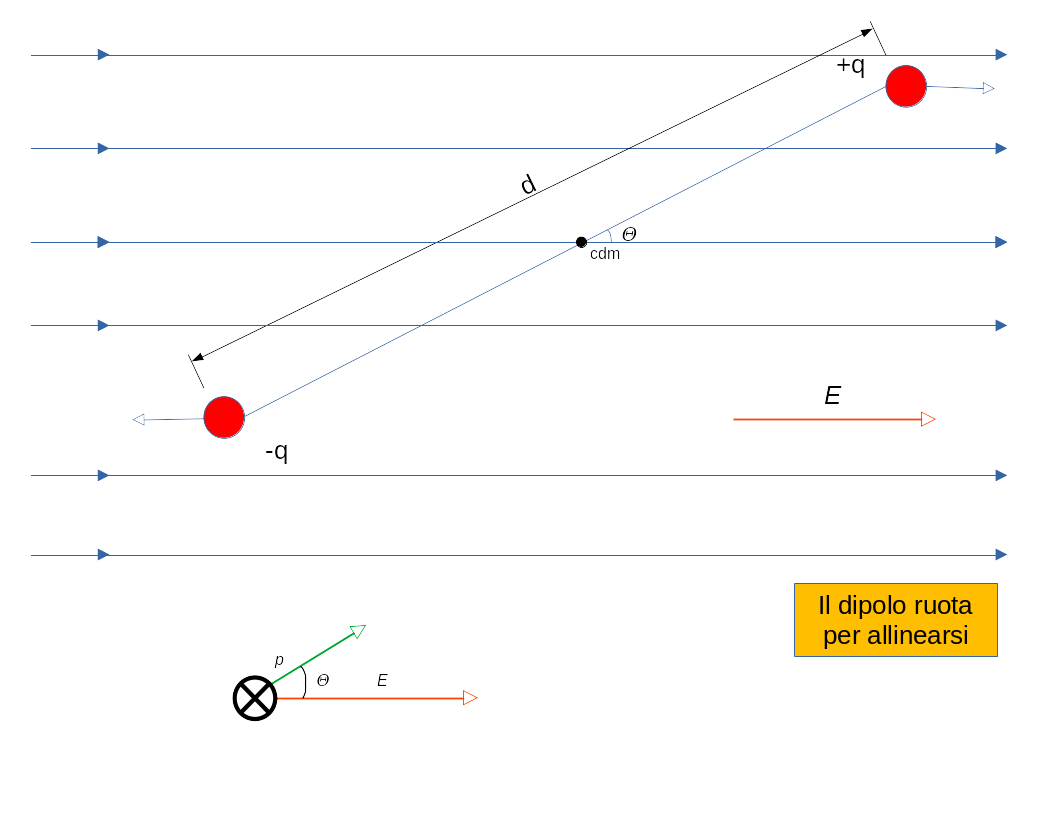
\includegraphics[height=8cm]{img/grafuci del dipolo elettrico.png}
\end{figure}
$\vec{F} (+q) e \vec{F} (-q)$ hanno intensità uguali e direzioni opposta. La forza netta è zero, ma esercitano un \textbf{momento torcente} $\vec{\uptau}$:
\begin{equation}
\uptau=-Fd \sin {\texttheta} = -pE sin {\texttheta}
\end{equation}
(\textit{segno meno perché il verso è orario}).
In forma vettore: $\vec{\uptau}=\vec{p}*\vec{E}$
\section{Energia potenziale di un dipolo elettrico}
L'energia potenziale $U$ di un dipolo elettrico $\vec{p}$ dipende dal suo \textit{orientamento}.
$U$ è minimo quando $\vec{p}$ è allineaTo Con il campo $\vec{E}$ - Nel mimimo è in equilibro:
$\abs{\vec{\uptau}}=\abs{p}\abs{E}\sin \texttheta=0$. Scegliamo $U=0$ per $\texttheta=90^o$.\\
L'energia potenziale diventa
\begin{equation}
  U=-L=\int^{\texttheta}_{90^o}\uptau d \texttheta= \int^{\texttheta}_{90^o} pE\sin \texttheta d\texttheta =-pE\cos\texttheta
\end{equation}
In forma vettoriale: $U=-\vec{p}*\vec{E}$
\section{Problema}
\begin{tasks}
  \task A quale distanza si trovano i cewntri delle cariche positiva e negativa di una molecola d'acqua?
  \begin{eqnarray*}
    p=qd\to d=\frac{p}{q}\\
    p(H_2O)=10e=1,6*10^{-30}C\\
    q(H_2O))10e)=1,6*10^{-18}C\\
    d=\frac{p}{q}=\frac{6,2*10^{-30}Cm}{1,6*10^{-18}C}=3,9*10^{-12}m=3,9pm
  \end{eqnarray*}
  \task Qual'è la differenza di energia potenziale tra le orientazioni $\texttheta=0^o$ e $\texttheta=180^o$ in un campo esterno $E=1,5*10^4\frac{N}{C}$?
  \begin{equation}
	\Delta U=2pE=2*6,2*10^{-30}Cm*1,5*10^3\frac{N}{C}=1,9*10^{-25}J
  \end{equation}
\end{tasks}
